\documentclass[12pt,a4paper,openany]{book}
\usepackage{lmodern}
\usepackage[svgnames]{xcolor} % Required to specify font color
\input{../LaTexTemplate/templates/couleurs.tex}

\usepackage{makeidx}
\usepackage[utf8]{inputenc} 
\usepackage{marvosym}
\usepackage[T1]{fontenc}
\usepackage[francais]{babel}
\usepackage[top=1.7cm, bottom=1.7cm, left=1.7cm, right=1.7cm]{geometry}
\usepackage{verbatim}
\usepackage[urlbordercolor={1 1 1}, linkbordercolor={1 1 1}, linkcolor=vert1, urlcolor=bleu, colorlinks=true]{hyperref}
\usepackage{tikz} %Vectoriel
\usepackage{listings}
\usepackage{fancyhdr}
\usepackage{multido}
\usepackage{amssymb}
\usepackage{slashbox}
\usepackage{float}
\usepackage[francais]{minitoc}
\usepackage[final]{pdfpages} 
\usepackage{pgfgantt}
\usepackage{graphicx} % Required for box manipulation
\usepackage{makeidx}
\usepackage{lscape}
\usepackage{rotating}
\usepackage{epstopdf}
\usepackage{lipsum}
\usepackage{wrapfig}


\newcommand{\titre}{Bilan du Projet}
\newcommand{\logoFooter}{\begin{minipage}{0.1\textwidth}
\includegraphics[width=2cm]{../../images/FACT_official.png}\end{minipage}}
\newcommand{\titreFooter}{Bilan du Projet FactDev} 
\newcommand{\subtitle}{FactDev} 
\newcommand{\auteur}{}
\newcommand{\semestre}{}
\newcommand{\annee}{2015}


\newcommand{\pole}{}
\newcommand{\sigle}{}
\newcommand{\FactDev}{\textit{FactDev}}
\newcommand{\key}[1]{\textit{#1}}
\newcommand{\Scrum}{\textit{Scrum}}
\newcommand{\UserStory}{\textit{User story}}
\newcommand{\UserStories}{\textit{User stories}}
\newcommand{\TechnicalStory}{\textit{Technical story}}
\newcommand{\TechnicalStories}{\textit{Technical stories}}
\newcommand{\Stories}{\textit{Stories}}
\newcommand{\Sprint}{\textit{Sprint}}
\newcommand{\Sprints}{\textit{Sprints}}
\newcommand{\PullRequest}{\textit{Pull Request}}
\newcommand{\Release}{\textit{Release}}
\newcommand{\Releases}{\textit{Releases}}
\newcommand{\Melee}{\textit{mêlée}}
\newcommand{\Melees}{\textit{mêlées}}
\newcommand{\Git}{\textit{Git}}
\newcommand{\Github}{\textit{Github}}
\newcommand{\Issue}{\textit{issue}}
\newcommand{\Issues}{\textit{issues}}
\newcommand{\Commit}{\textit{commit}}
\newcommand{\Commits}{\textit{commits}}
\newcommand{\Travis}{\textit{Travis CI}}
\newcommand{\Coveralls}{\textit{Coveralls}}
\newcommand{\SonarQube}{\textit{SonarQube}}
\newcommand{\BurnUp}{\textit{BurnUp Chart}}
\newcommand{\Backlog}{\textit{Backlog}}
\newcommand{\PlanningPoker}{\textit{Planning Poker}}
\newcommand{\Build}{\textit{Build}}
\newcommand{\Refactoring}{\textit{Refactoring}}
\newcommand{\approved}{true}

\makeindex
\usepackage[totoc]{idxlayout}


\input{../LaTexTemplate/templates/listings.tex}
\input{../LaTexTemplate/templates/classroomsTemplates/l3/cours.tex}
\input{../LaTexTemplate/templates/remarquesExempleAttention.tex}
\input{../LaTexTemplate/templates/polices.tex}
\input{../LaTexTemplate/templates/affichageChapitre.tex}


\newcommand*{\plogo}{\fbox{$\mathcal{PL}$}} % Generic publisher logo
%----------------------------------------------------------------------------------------
%	TITLE PAGE
%----------------------------------------------------------------------------------------

\newcommand*{\rotrt}[1]{\rotatebox{90}{#1}} % Command to rotate right 90 degrees
\newcommand*{\rotlft}[1]{\rotatebox{-90}{#1}} % Command to rotate left 90 degrees

\newcommand*{\titleBC}{\begingroup % Create the command for including the title page in the document
\newlength{\drop} % Command for generating a specific amount of whitespace
\drop=0.1\textheight % Define the command as 10% of the total text height

\vspace*{-50px}
\rule{\textwidth}{0.4pt}\par % Thick horizontal line
\begin{tabular}{p{8cm}p{5cm}p{6cm}}
	\begin{minipage}{8cm}
		Équipe FACT\\
		\textit{Conception et développement d'applications}\\~\\
		\small
%		\Mobilefone~06~84~33~52~93\\
%		\Letter~\texttt{antoine.roquemaurel@gmail.com}\\
		\Mundus~\url{http://fact-team.github.io}
	\end{minipage} &
	& 

	\begin{minipage}{5cm}
		\begin{center}
			
\includegraphics[width=5cm]{logo.jpg}\\
			\tiny{Rédigé avec \LaTeX{}\\Version du \today}
		\end{center}
	\end{minipage}
\end{tabular}

\vspace{\drop} % Whitespace between the top lines and title
\centering % Center all text

\vspace{100px}
\def\CP{\textit{\Huge \titre}} % Title

\settowidth{\unitlength}{\CP} % Set the width of the curly brackets to the width of the title
{\color{LightGoldenrod}\resizebox*{\unitlength}{\baselineskip}{\rotrt{$\}$}}} \\[\baselineskip] % Print top curly bracket
\textcolor{Sienna}{\CP} \\[\baselineskip] % Print title
{\color{RosyBrown}\Large \subtitle} \\ % Tagline or further description
{\color{LightGoldenrod}\resizebox*{\unitlength}{\baselineskip}{\rotlft{$\}$}}} % Print bottom curly bracket

\vfill % Whitespace between the title and the author name


{
\normalsize \LARGE Université Toulouse III -- Paul Sabatier}\\ % Author name

\vfill % Whitespace between the author name and the publisher logo
\Large \today % Year published

\rule{\textwidth}{0.4pt}\par % Thick horizontal line

\endgroup}

%----------------------------------------------------------------------------------------
%	BLANK DOCUMENT
%----------------------------------------------------------------------------------------


\makeatother
\includeonly {
contents/preambule,
contents/projet,
contents/methodologie,
contents/resultats,
contents/conclusion
}
\begin{document}
	\thispagestyle{empty} % Removes page numbers
	\titleBC
	\dominitoc
	\setcounter{tocdepth}{1}
	\setcounter{secnumdepth}{3}
	\setcounter{minitocdepth}{1}
	
	\tableofcontents
	
	\chapter*{Introduction}

\setlength{\parindent}{1cm}
\FactDev{}  est un logiciel de devis et de facturation réalisé dans le cadre de l’UE Projet. 

Ce projet s’est fait en réponse à un problème de l’un des membres du groupe : Antoine De Roquemaurel. En effet Antoine, développeur \textit{Freelance}, rédigeait pour ses clients les factures et devis « à la main ». La tâche était répétitive et le risque d’erreurs humaine important : 
\begin{itemize}
	\item erreur dans le calcul des montants
	\item perte de facture
	\item plusieurs factures différentes pour un même projet et donc risque de ne pas faire le bon travail demandé par le client
\end{itemize}

Face à ces difficultés, Antoine a soumis le projet devant répondre aux spécifications suivantes :
\begin{itemize}
	\item Gestion des clients
	\item Gestion des projets associées aux clients
	\item Calculs des tarifs
	\item Génération de documents
	\item Recherche
\end{itemize}


Les autres membres ont vu dans ce projet l'opportunité de développer de nouvelles compétences, aussi bien sur le plan technique qu'organisationnel. D'un point de vue technique avec l'utilisation du \textit{LaTeX} et du \textit{C++} accompagné du \textit{framework Qt}. Sur le plan organisationnel avec la mise en place de la méthode Agile \Scrum. 

Ce document fait état des parties prenantes, des outils et des méthodologies de développement appliquées au projet. Il fait le point sur les résultats obtenus au niveau de la méthodologie, du logiciel et en terme de respect du plan qualité. 
	\chapter{Le projet}
\section{Le logiciel FactDev}


\section{Les outils}
Afin de respecter les attentes du client, et de développer correctement le logiciel présenté section \ref{logiciel}, nous avons utilisés un
certain nombres d'outils, dans divers domaines.

\subsection{Outils de développement}
Afin de développer à proprement parler le logiciel, nous avons utilisés plusieurs technologies. 

\begin{wrapfigure}{r}{0.4\textwidth}
\begin{center}

\includegraphics[width=0.38\textwidth]{../beamer/logos/qt.png}
\end{center}
\caption{Le développement -- Qt}
\end{wrapfigure}
Proposé par le client, il a été choisi de développer le logiciel en C++, en utilisant le framework Qt. 
En effet, ce langage permet d'avoir un logiciel qui soit rapide, et peu gourmand en mémoire. Cependant, il était nécessaire d'utiliser un
framework de développement, et ce pour plusieurs raisons : 
\begin{itemize}
	\item Développer rapidement une interface claire, uniforme
	\item Avoir un logiciel Multi-Plateforme, executable sous Windows, Linux et Mac OS
	\item Faciliter les lectures et écritures à une base de données 
\end{itemize}
En plus de ces avantages certains, Qt améliore le langage C++ afin de garder la même rapidité d'exécution tout en simplifiant l'écriture de
certains concepts\footnote{Simplification de la gestion de la mémoire, Ajout du \textit{foreach}, redéfinition de tous les types de bases, …}.

\newpage
\begin{wrapfigure}{l}{0.3\textwidth}
\begin{center}
	\Huge \LaTeX
\end{center}
\caption{La mise en formex -- \LaTeX}
\end{wrapfigure}
Un des besoins du client, était la génération des factures et des devis au format PDF. Avant le développement du logiciel, ce besoin était
fait << à la main >>, en \LaTeX{}, avec un \textit{template} rédigé. Afin de regarder la même mise en forme des devis et des factures, nous
devions générer du \LaTeX{} en réutilisant ce template.\\ Une fois ce fichier \texttt{.tex} généré, nous faisons appel à un compilateur \LaTeX{} afin d'en sortir un fichier PDF.

\begin{wrapfigure}{r}{0.4\textwidth}
\begin{center}

\includegraphics[width=0.18\textwidth]{../beamer/logos/sqlite.png}~

\includegraphics[width=0.18\textwidth]{../beamer/logos/mysql.png}
\end{center}
\caption{Bases de données}
\end{wrapfigure}
Le logiciel utilise une base de données pour sauvegarder les différents clients, devis, factures etc… Le besoin initial était de pouvoir
sauvegarder ça sur un ordinateur : le système de SQLite permet cela très simplement, tout est sauvegardé dans un fichier binaire.\\ Une fois
avancé dans le projet, une autre solution est apparu : posséder un serveur de base de données afin d'utiliser le logiciel avec plusieurs
postes clients. Ce besoin a été couvert à l'aide de MySQL, ainsi le logiciel permet de choisir l'une ou l'autre des manières de procéder.


\subsection{Versionnement}


\subsection{Qualité du code}


\subsection{Organisation}


	\section{La méthodologie}

	\chapter{Les résultats}
\section{La méthodologie}

\section{Le logiciel FactDev}



	\chapter*{Conclusion}
	\appendix
	\chapter{Conventions de programmation en C++}
Voici les conventions d'écriture que nous avons fixé, il faudra les
respecter pour que nous ayons un code propre et homogène, de plus elles
ont été fixées pour que ce soit le plus simple pour nous (lecture rapide,
propreté etc\ldots{}).

\begin{attention}
Elles peuvent encore évoluer
\end{attention}

\section{English, of course !}\label{english-of-course}

Tout le code, et les \texttt{commits}, doivent être rédigés en Anglais. Soit, les
noms de classes, de méthodes, de fichiers, de variables, d'attributs, et
même les commentaires ;-) C'est pas compliqué, mais au moins, on se met
tous d'accord, et puis voilà :)

\section{Le nommage}\label{le-nommage}

\subsection{Les attributs}\label{les-attributs}

Les attributs doivent toujours commencer avec une minuscule, pour
séparer les mots, on les sépare avec une majuscule : utilisation de la
Camel Case. Les noms de variables claires et explicite, quitte à ce
qu'il soit un peu long, on a l'auto complétion que diable! Donc les
variables d'une lettre, à bannir! (à part le i dans le cas d'un for,
s'il n'est pas réutilisé après le for)

Les attributs seront préfixés par \texttt{\_} afin de pouvoir les reconnaître
facilement.

\begin{lstlisting}[language=C++,numbers=none]
int _superField; 
bool _youLostTheGame;
\end{lstlisting}

\subsection{Les noms de constantes}\label{les-noms-de-constantes}

Les constantes doivent être tout en majuscule, les différents mots de la
constante sont séparés par des underscore (\texttt{\_}). Même remarque que pour
les attributs, choisissez des noms de constantes clairs, compréhensibles
par tous, pas seulement par ceux qui sont dans votre tête!

\begin{lstlisting}[language=C++]
const int MY_BEAUTIFUL_CONSTANT; 
const bool YOU_LOST_THE_GAME_AGAIN; 
const QString CONST;
\end{lstlisting}

\begin{exemple}
	On évite d'utiliser les \texttt{\#define} afin de garder un typage fort
\end{exemple}

\subsection{Les noms de méthodes}\label{les-noms-de-muxe9thodes}

Les méthodes doivent commencer par une minuscule, et séparer les
différents mots par une majuscule(Camel case).

Les fonctions ne retournant rien (procédures) doivent toujours être à
l'infinitif.

\`A l'opposé les fonctions 
retournant quelques choses doivent être au
participe passé. Il faut décomposer au maximum, n'hésitez pas à faire
une méthode \texttt{private} si besoin est, c'est toujours plus clair
d'avoir une fonction, dictant explicitement ce qu'elle fait par son nom
que 10 lignes de code bizarroïdes avec 2-3 lignes de commentaire! Et donc, les noms de fonctions sont essentiels!!

\begin{lstlisting}[language=C++]
void display(QString textToDisplay) { 
    qDebug() << texteAAffiche; 
}

bool test(int first, int second) { 
	return (first + second);
} 
\end{lstlisting}

\paragraph{Les accesseurs}\label{les-accesseurs}

Les getters et les setters doivent être respectivement préfixés par
\texttt{get} et \texttt{set} suivi du nom \emph{exact} de l'attribut,
même si le get ne respecte pas la convention de Qt.

\begin{lstlisting}[language=C++]
int getValue(); 
void setValue(int);
\end{lstlisting}

\subsection{Les noms de classes ou d'interface}\label{les-noms-de-classes-ou-dinterface}

Les noms de classe ou d'interface doivent tous commencer par une
majuscule, les différents mots sont séparés par une majuscule,
choisissez des noms de classes claires! (oui, je me répète, mais c'est
ce qui fait toute la compréhension facile, ou non, d'un programme les
noms de variables, classe, paramètre, méthodes etc\ldots{} )

\section{L'indentation}\label{lindentation}

La règle est simple, on ouvre une accolade, la ligne suivante sera
décalée vers la droite(une tab = 4 caractères), on ferme une accolade, on
décale l'accolade vers la gauche et tout ce qui suit.

Également, si une ligne est trop longue, on va à la ligne, et décalons
d'une ligne vers la droite, une fois l'instruction finie, on redécale
vers la gauche.

Dans le cas d'un switch, le break doit s'aligner avec le case 42: tout
ce qui est entre case et break sera indenté.

Merci de mettre un espace avant chaque accolade, oui je sais je suis
psychorigide, mais c'est moche sinon.

\begin{lstlisting}[language=C++]
class MaSuperClasse { 
public: 
	MaSuperClasse(int test, QString, machin, double _chose);
	int method();

private: 
	int _test;
	QString _machin;
	double _chose;
};

MaSuperClasse::MaSuperClasse(int test, QString machin, double chose) {
	_test = test;
	_machin = machin; 
	_chose = chose; 
}

MaSuperClasse::method() {
	qDebug() << "Hello World";
	switch(yatta) {
		case 42:
		   // ^^
		   break;
		case 1337:
		   // ...
		   break;
		default: 
		   //
	}
}
\end{lstlisting}

\section{Les accolades}\label{les-accolades}

Les accolades ouvrantes sont positionnées à la fin de la ligne demandant
une accolade (\texttt{switch}, \texttt{if}, \texttt{class}, \texttt{else}, \texttt{else if}, \ldots{})

Les accolades fermantes sont positionnées une ligne après la dernière
instruction. (avec une désindentation) Les \texttt{else} et \texttt{else if} se mettent sur la 
même ligne que l'accolade fermante.


\begin{lstlisting}[language=C++]
int superMethod(void) {     
	if(true) {
		// bla bla     
	} else if(false) {
		// bla bla      
	} else { 
		//instruction 
	}
}
\end{lstlisting}

\section{Les types}\label{les-types}

Pour les types, au maximum, il vaut mieux privilégier les classes de Qt
plutôt que les Types C++, autrement dit, on va utiliser les types
suivants(c'est facile, ça commence pas un Q :) ) :

\begin{itemize}
\itemsep1pt\parskip0pt\parsep0pt
\item
  Primitives : \texttt{int}, \texttt{double}, \texttt{char},
  \texttt{unsigned}, \texttt{bool}, \ldots{}
\item
  \texttt{QString}, \texttt{QVariant}, \texttt{QNumber}, \texttt{QDate},
  \texttt{QTime}, \texttt{QDateTime}
\item
  Collections : \texttt{QList\textless{}Type\textgreater{}},
  \texttt{QSet\textless{}Type\textgreater{}},
  \texttt{QStack\textless{}Type\textgreater{}},
  \texttt{QQueue\textless{}Type\textgreater{}},
  \texttt{QLinkedList\textless{}Type\textgreater{}},
  \texttt{QVector\textless{}Type\textgreater{}},
  \texttt{QMap\textless{}Type1, Type2\textgreater{}} \ldots{}
\end{itemize}

Je vous ferais p'têtre un wiki sur les types cool en Qt\ldots{} Mais
sinon la doc est vraiment très bien faite ! Au pire, c'est assez intuitif
« je veux une pile\ldots{} Ça commence par Q. Comment on dit pile ?
Stack ? Ah ben \texttt{QStack}. »

\section{Les bonnes pratiques}\label{les-bonnes-pratiques}

\subsection{Le mot clé \texttt{const}}\label{le-mot-cluxe9-const}

Dès que vous pouvez\ldots{} hop un \texttt{const}.

Autrement dit : si vous ne modifiez jamais un paramètre, un attribut, une
variable où que sait-je, on met un const. Ça permet de n'avoir aucune
ambiguïté, c'est clair, et quelqu'un qui utilise la méthode sait que le
paramètre ne serait pas modifié.

\subsection{Le mot clé \texttt{void}}\label{le-mot-cluxe9-void} 
Une méthode ne contenant aucun paramètre \emph{doit} contenir void,
c'est comme ça.

\begin{lstlisting}[language=C++,numbers=none]
void aSuperMethod(void);
\end{lstlisting}

\subsection{Longueur du code}\label{longueur-du-code}

Une ligne ne doit pas excéder 100 caractères, une méthode ne doit pas
excéder 60 lignes, un fichier doit être assez court\ldots{} Mais ça on
verra sur le moment ;-)

\section{Conventions des composants
graphiques}\label{conventions-des-composants-graphiques}
\begin{tabular}{c|c}
Element & Préfix\\
\hline
Combo & cb\\
Menus & mn\\
LineEdit & le\\
Buttons & btn\\
Table & tbl\\
Label & lb\\
TextEdit & te\\
Tree & tr\\
Dock & dck\\
Checkbox & chk\\
WIdget & wdg\\
\end{tabular}

\section{Conventions de documentation}\label{conventions-de-documentation}

\subsubsection{Pour une classe}\label{pour-une-classe}


\begin{lstlisting}[language=C++,numbers=none]
/**
 * @author Nom de(s) la personne ayant programmé la classe sous la forme: Prénom Nom
 * @brief The MaClass class (généré automatiquement) Role de la classe 
 */
\end{lstlisting}

\subsubsection{Pour un attribut ou une méthode}
\begin{lstlisting}[language=C++,numbers=none]
/**
 * @brief MaClass\dotsmaMethode Ce que fait la méthode
 * @see [optionnelle] Si cela fait référence à une autre méthode/classe/objet alors on écrit le nom de cette
 * méthode/classe/objet
 * @param parametre1 Brève description du paramètre attendu et de ce qu'il représente 
 * @param parametre2 \ldots
 * @param parametreN \ldots
 * @return ce qui est retourné
 */
\end{lstlisting}

\subsubsection{Remarques}
On peut utiliser les balises HTML pour la documentation. Par exemple, dans @brief si on a une méthode addCustomer(int id), sa description pourrait
être: 
\begin{lstlisting}[language=C++,numbers=none]
/**
 * @brief Customer\dotsaddCustomer Ajoute un nouveau client 
 *  possédant l'identifiant <i>id</i>``. 
 */
\end{lstlisting}

On utilisera alors comme convention: - Pour un paramètre << pParam >> passé en paramètre: 
\begin{lstlisting}[language=C++,numbers=none]
/**
 * ...<i>pParam</i>
 */
\end{lstlisting}

- Pour le nom d'une classe << MaClass >> 
\begin{lstlisting}[language=C++,numbers=none]
/**
 * ...<b>MaClass</b>
 */
\end{lstlisting}

\begin{attention}
Éviter les accents dans la documentation (Par exemple, ça sera @author Cedric Rohaut et non Cédric Rohaut)
\end{attention}

	\chapter{Backlog product}\label{backlog}
	\begin{sidewaysfigure}[ht]
		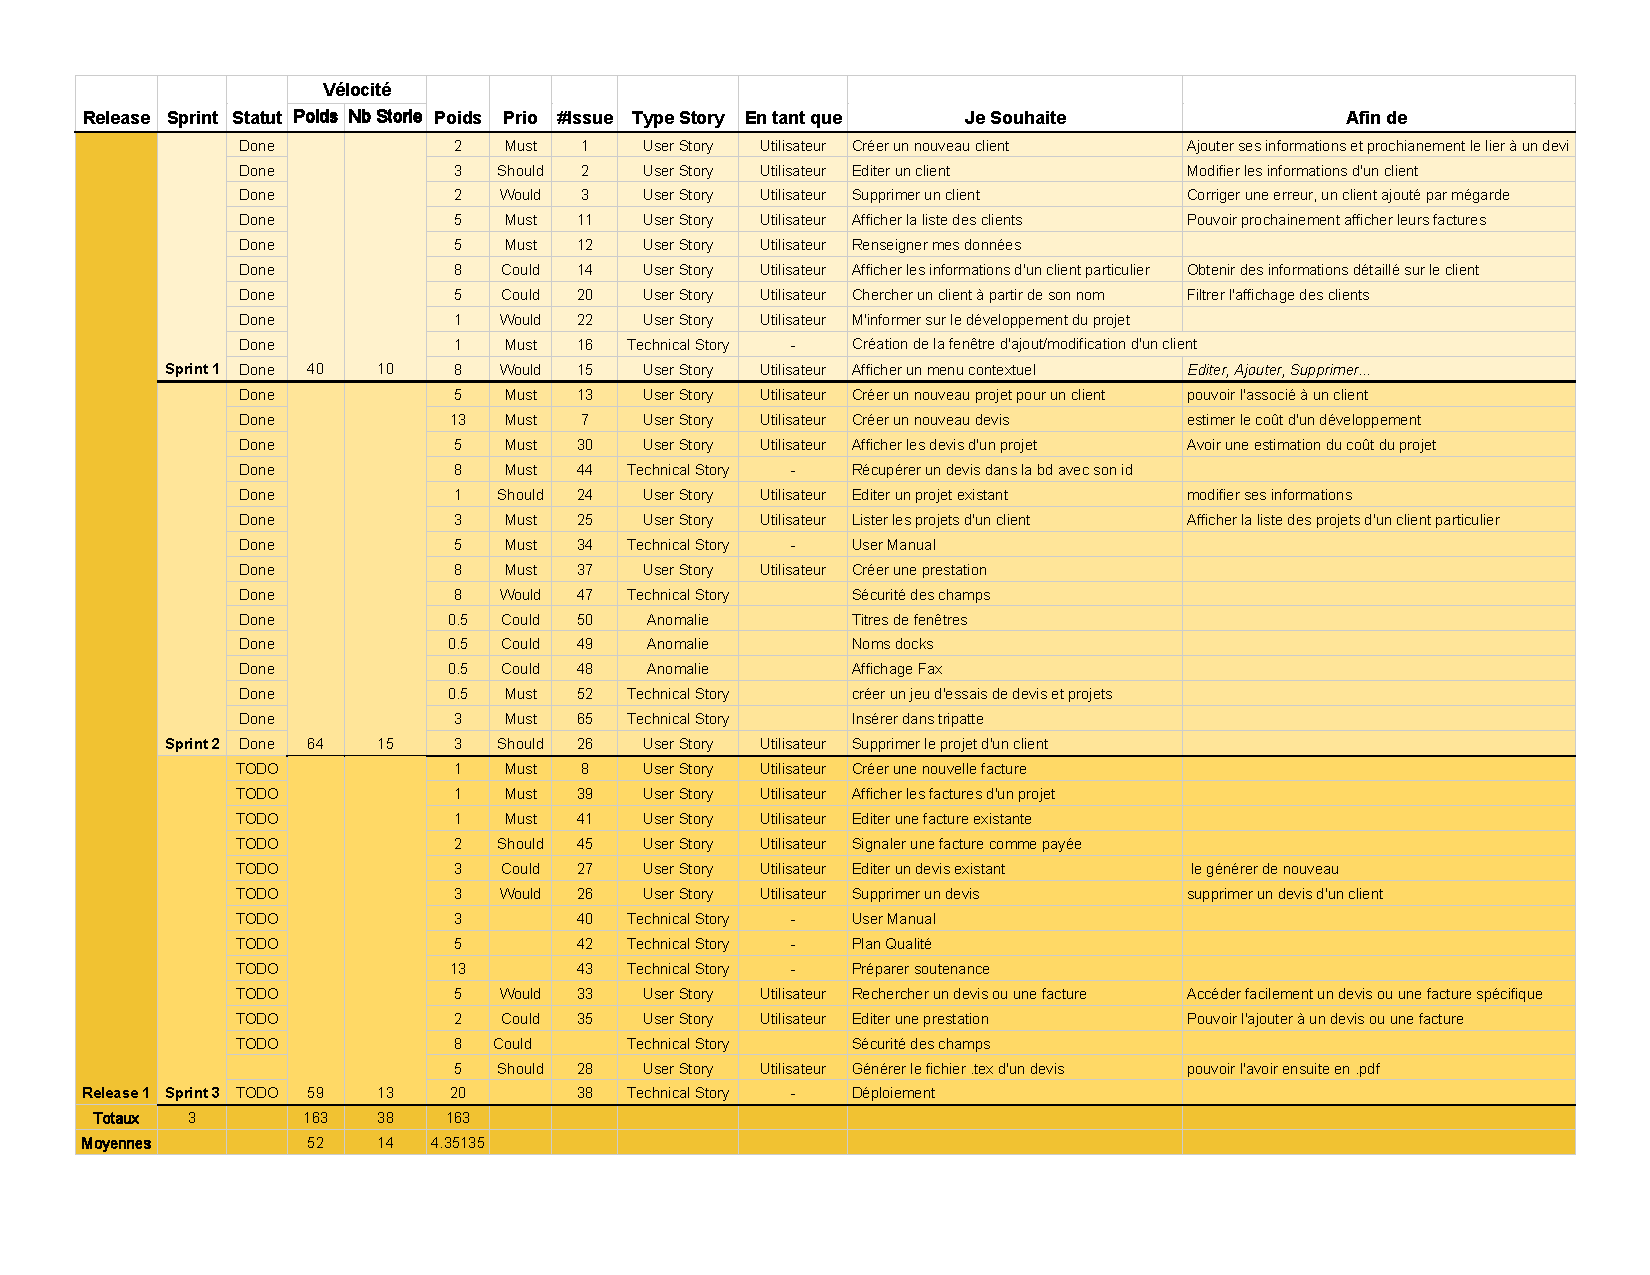
\includegraphics{backlog.pdf}
	\end{sidewaysfigure}
	\chapter{Références}
\begin{description}
	\item[\Mundus~\url{http://fact-team.github.io/}] Site web de l'équipe FACT
	\item[\Mundus~\url{http://fact-team.github.io/doc/html/index.html}] Documentation \bsc{html} du projet
	\item[\Mundus~\url{https://github.com/FACT-Team/FactDev}] Code source du projet
	\item[\Mundus~\url{https://travis-ci.org/FACT-Team/FactDev}] Intégration continue du projet
	\item[\Mundus~\url{https://coveralls.io/r/FACT-Team/FactDev}] Couverture de code
	\item[\Mundus~\url{https://github.com/FACT-Team/FactDev/wiki}] Wiki de FactDev
\end{description}

	\listoffigures
	\printindex

\end{document}
